\documentclass[12pt,letterpaper]{article}
\usepackage{graphicx,textcomp}
\usepackage{natbib}
\usepackage{setspace}
\usepackage{fullpage}
\usepackage{color}
\usepackage[reqno]{amsmath}
\usepackage{amsthm}
\usepackage{fancyvrb}
\usepackage{amssymb,enumerate}
\usepackage[all]{xy}
\usepackage{endnotes}
\usepackage{lscape}
\newtheorem{com}{Comment}
\usepackage{float}
\usepackage{hyperref}
\newtheorem{lem} {Lemma}
\newtheorem{prop}{Proposition}
\newtheorem{thm}{Theorem}
\newtheorem{defn}{Definition}
\newtheorem{cor}{Corollary}
\newtheorem{obs}{Observation}
\usepackage[compact]{titlesec}
\usepackage{dcolumn}
\usepackage{tikz}
\usetikzlibrary{arrows}
\usepackage{multirow}
\usepackage{xcolor}
\newcolumntype{.}{D{.}{.}{-1}}
\newcolumntype{d}[1]{D{.}{.}{#1}}
\definecolor{light-gray}{gray}{0.65}
\usepackage{url}
\usepackage{listings}
\usepackage{color}

\definecolor{codegreen}{rgb}{0,0.6,0}
\definecolor{codegray}{rgb}{0.5,0.5,0.5}
\definecolor{codepurple}{rgb}{0.58,0,0.82}
\definecolor{backcolour}{rgb}{0.95,0.95,0.92}

\lstdefinestyle{mystyle}{
	backgroundcolor=\color{backcolour},   
	commentstyle=\color{codegreen},
	keywordstyle=\color{magenta},
	numberstyle=\tiny\color{codegray},
	stringstyle=\color{codepurple},
	basicstyle=\footnotesize,
	breakatwhitespace=false,         
	breaklines=true,                 
	captionpos=b,                    
	keepspaces=true,                 
	numbers=left,                    
	numbersep=5pt,                  
	showspaces=false,                
	showstringspaces=false,
	showtabs=false,                  
	tabsize=2
}
\lstset{style=mystyle}
\newcommand{\Sref}[1]{Section~\ref{#1}}
\newtheorem{hyp}{Hypothesis}

\title{Problem Set 3}
\date{Due: November 20, 2022}
\author{Applied Stats/Quant Methods 1: 16327268, Marcus Ó Faoláin}


\begin{document}
	\maketitle
	\section*{Instructions}
	\begin{itemize}
		\item Please show your work! You may lose points by simply writing in the answer. If the problem requires you to execute commands in \texttt{R}, please include the code you used to get your answers. Please also include the \texttt{.R} file that contains your code. If you are not sure if work needs to be shown for a particular problem, please ask.
	\item Your homework should be submitted electronically on GitHub.
	\item This problem set is due before 23:59 on Sunday November 20, 2022. No late assignments will be accepted.
	\item Total available points for this homework is 80.
	\end{itemize}

		\vspace{.25cm}
	
\noindent In this problem set, you will run several regressions and create an add variable plot (see the lecture slides) in \texttt{R} using the \texttt{incumbents\_subset.csv} dataset. Include all of your code.

	\vspace{.5cm}
\section*{Question 1}
\vspace{.25cm}
\noindent We are interested in knowing how the difference in campaign spending between incumbent and challenger affects the incumbent's vote share. 
	\begin{enumerate}
		\item Run a regression where the outcome variable is \texttt{voteshare} and the explanatory variable is \texttt{difflog}.	\vspace{5cm}
		\item Make a scatterplot of the two variables and add the regression line. 	\vspace{7cm}
		\item Save the residuals of the model in a separate object.	\vspace{7cm}
		\item Write the prediction equation.
	\end{enumerate}
	
\newpage

\section*{Question 1}
\vspace{.25cm}
\noindent We are interested in knowing how the difference in campaign spending between incumbent and challenger affects the incumbent's vote share. 
\begin{enumerate}
	\item Run a regression where the outcome variable is \texttt{voteshare} and the explanatory variable is \texttt{difflog}.	
\\\\
\noindent We run a regression where \texttt{voteshare} is the outcome variable (Y) and \texttt{difflog} is the explanatory variable (X). We save it in a variable \texttt{voteshare.difflog.lm} and use the \texttt{summary()} function to view the results. Finally, we generate Latex output using \texttt{stargazer} which generates the table below.
\begin{lstlisting}
voteshare.difflog.lm <- lm(voteshare ~ difflog, data = data)
summary(voteshare.difflog.lm)
stargazer(voteshare.difflog.lm, type='latex', summary= FALSE)
\end{lstlisting}
\begin{table}[!htbp] \centering 
  \caption{} 
  \label{} 
\begin{tabular}{@{\extracolsep{5pt}}lc} 
\\[-1.8ex]\hline 
\hline \\[-1.8ex] 
 & \multicolumn{1}{c}{\textit{Dependent variable:}} \\ 
\cline{2-2} 
\\[-1.8ex] & voteshare \\ 
\hline \\[-1.8ex] 
 difflog & 0.042$^{***}$ \\ 
  & (0.001) \\ 
  & \\ 
 Constant & 0.579$^{***}$ \\ 
  & (0.002) \\ 
  & \\ 
\hline \\[-1.8ex] 
Observations & 3,193 \\ 
R$^{2}$ & 0.367 \\ 
Adjusted R$^{2}$ & 0.367 \\ 
Residual Std. Error & 0.079 (df = 3191) \\ 
F Statistic & 1,852.791$^{***}$ (df = 1; 3191) \\ 
\hline 
\hline \\[-1.8ex] 
\textit{Note:}  & \multicolumn{1}{r}{$^{*}$p$<$0.1; $^{**}$p$<$0.05; $^{***}$p$<$0.01} \\ 
\end{tabular} 
\end{table} 
\newpage
\noindent Attached is a screenshot of the console output when we run a summary call on the \texttt{voteshare.difflog.lm} model.

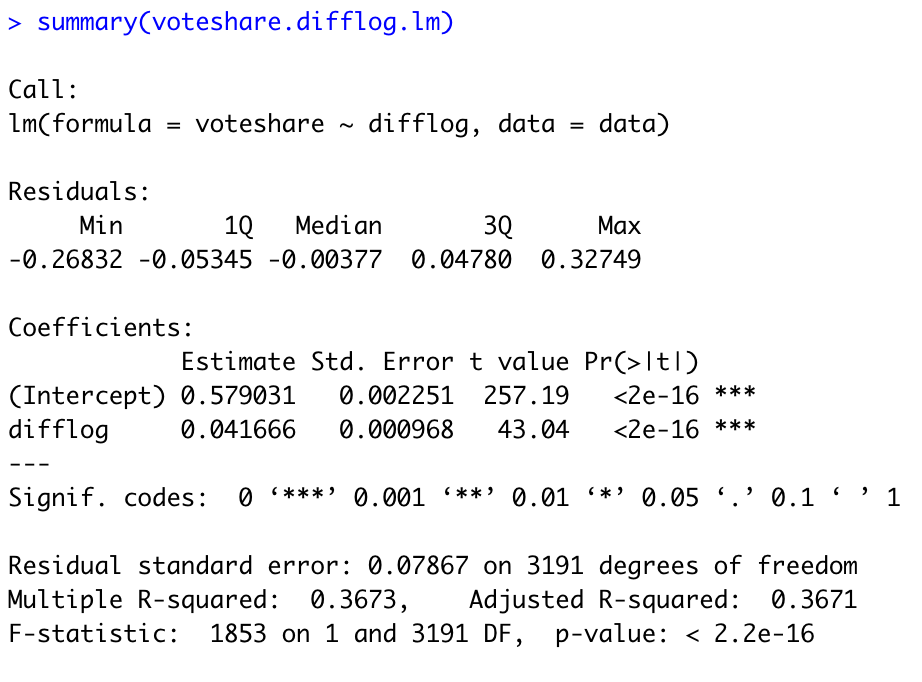
\includegraphics{PS3 Q1 Regression.png}
\\\\
\noindent The residuals are the difference between the predicted and observed values in the model. The min value for these residuals is -0.26832 and the max value is 0.32749. The median -0.00377 is quite close to 0, which suggests that the residuals are somewhat symmetrical. 
\\\\
\noindent The low and signficant p-values in our model for the intercept and for the coefficient \texttt{difflog} suggest that the coefficient is not zero and suggest that there is strong evidence that it explains variance in our model.
\\\\
\noindent The Multiple R-squared value of this simple linear regression gives us an indication of how much of the outcome variable is explained by the explanatory variable. The Multiple R-squared value of 0.3673 suggests that 36.73 percent of the variation in voteshare is explained by the explanatory variable difflog.
\\\\
\noindent Finally, the low p-value well below 0.05 suggests that there is strong evidence that the coefficient in this model isn't 0, and that the \texttt{difflog} variable does have an effect on \texttt{voteshare}

\newpage


\item Make a scatterplot of the two variables and add the regression line. 
\\\\
\noindent We use the ggplot() function to create the scatterplot where the \texttt{difflog} is on the x axis and \texttt{voteshare} is on the y axis. We use the \texttt{geom smooth(method=lm)} function to generate the regression line.
\begin{lstlisting}
ggplot(data, aes(x=difflog, y=voteshare))+
geom_point()+
geom_smooth(method=lm)
\end{lstlisting}
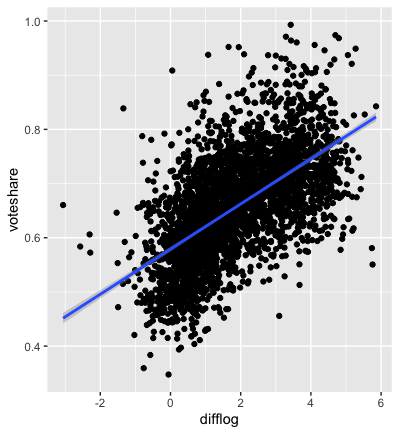
\includegraphics{Scatterplot Difflog Voteshare.png}
\newpage
\item Save the residuals of the model in a separate object.	
\\\\
\noindent We save the residuals in a separate variable by running the regression again and assigning the residuals portion of the regression to a variable using \texttt{resid}.
\begin{lstlisting}
residualsVoteshareDifflog <- lm(voteshare ~ difflog, data = data)$resid
residualsVoteshareDifflog
\end{lstlisting}

\item Write the prediction equation.
\\\\
\noindent The formula for the prediction equation is \texttt{y = b0 + b1x}, where b0 is the intercept of the regression and b1, the coefficient of x, is the \texttt{difflog} value in the regression.
\\\\
\noindent As we can see from Table 1, the value for \texttt{difflog} (b1) is 0.042 and the value of the intercept (b0) of the regression is 0.579.
\\\\
\noindent Therefore, the prediction equation is \texttt{y = 0.042x + 0.579}.


\end{enumerate}

\newpage

\section*{Question 2}
\noindent We are interested in knowing how the difference between incumbent and challenger's spending and the vote share of the presidential candidate of the incumbent's party are related.	\vspace{.25cm}
	\begin{enumerate}
		\item Run a regression where the outcome variable is \texttt{presvote} and the explanatory variable is \texttt{difflog}.	

\noindent	We run a regression where the outcome variable (Y) is \texttt{presvote} and the explanatory variable (x) is \texttt{difflog}. We save it in a variable called \texttt{presvote.difflog.lm} and use the summary function to view the results. Finally, we generate Latex output using \texttt{stargazer}, which generate the below output.
\begin{lstlisting}
presvote.difflog.lm <- lm(presvote ~ difflog, data = data)
summary(presvote.difflog.lm)
stargazer(voteshare.difflog.lm, type='latex', summary= FALSE)
\end{lstlisting}
\begin{table}[!htbp] \centering 
  \caption{} 
  \label{} 
\begin{tabular}{@{\extracolsep{5pt}}lc} 
\\[-1.8ex]\hline 
\hline \\[-1.8ex] 
 & \multicolumn{1}{c}{\textit{Dependent variable:}} \\ 
\cline{2-2} 
\\[-1.8ex] & presvote \\ 
\hline \\[-1.8ex] 
 difflog & 0.024$^{***}$ \\ 
  & (0.001) \\ 
  & \\ 
 Constant & 0.508$^{***}$ \\ 
  & (0.003) \\ 
  & \\ 
\hline \\[-1.8ex] 
Observations & 3,193 \\ 
R$^{2}$ & 0.088 \\ 
Adjusted R$^{2}$ & 0.088 \\ 
Residual Std. Error & 0.110 (df = 3191) \\ 
F Statistic & 307.715$^{***}$ (df = 1; 3191) \\ 
\hline 
\hline \\[-1.8ex] 
\textit{Note:}  & \multicolumn{1}{r}{$^{*}$p$<$0.1; $^{**}$p$<$0.05; $^{***}$p$<$0.01} \\ 
\end{tabular} 
\end{table}
\newpage
\noindent Attached below is a screenshot of the output generated when the summary call is used on the \texttt{presvote.difflog.lm} regression.
\\\\
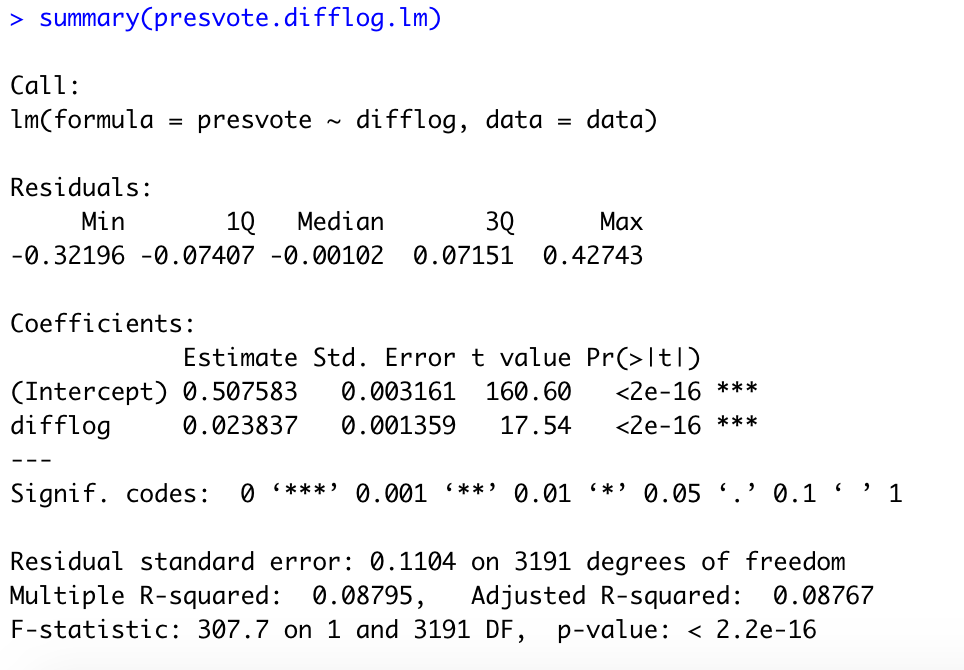
\includegraphics{PS3 Q2 Regression}

\newpage
		\item Make a scatterplot of the two variables and add the regression line.
\\\\
\noindent We use the ggplot() function to create the scatterplot where \texttt{difflog} is on the x axis and \texttt{presvote} is on the y axis. We use the \texttt{geom smooth(method = lm)} function to generate a regression line
\begin{lstlisting}
ggplot(data, aes(x=difflog, y=presvote))+
geom_point()+
geom_smooth(method=lm)
\end{lstlisting}
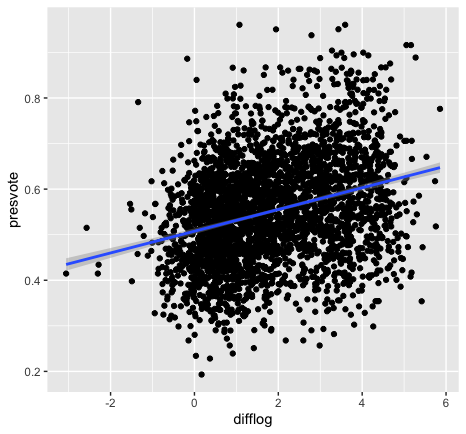
\includegraphics{Scatterplot Difflog Presvote.png}		

\newpage
		\item Save the residuals of the model in a separate object.	
\\\\
\noindent We save the residuals of the regression into a separate variable by selecting the \texttt{resid} portion of the regression and assigning it to a new variable.

\begin{lstlisting}
residualsPresvoteDifflog <- lm(presvote ~ difflog, data = data)$resid
residualsPresvoteDifflog
\end{lstlisting}		

		\item Write the prediction equation.
\\\\
\noindent As in Question 1, the prediction equation is given by \texttt{y = b0 + b1x}, where b0 is the intercept of the regression and b1, the coefficient of x, is the \texttt{difflog} value in the regression.
\\\\
\noindent As we can see in Table 2, the value for \texttt{difflog} (b1) is 0.024 and the value of the intercept (b0) is 0.508.
\\\\
\noindent Therefore the prediction equation is:
\\\\
\noindent \texttt{y = 0.024x + 0.508}.

	\end{enumerate}
	
	\newpage

	
		
\section*{Question 3}

\noindent We are interested in knowing how the vote share of the presidential candidate of the incumbent's party is associated with the incumbent's electoral success.
	\vspace{.25cm}
	\begin{enumerate}
		\item Run a regression where the outcome variable is \texttt{voteshare} and the explanatory variable is \texttt{presvote}.
\\\\
\noindent We run a regression where the outcome variable (y) is \texttt{voteshare} and the explanatory variable (x) is \texttt{presvote}. We save it in a variable called \texttt{voteshare.presvote.lm} and use the summary function to view the results. Finally, using the \texttt{stargazer} function we generate the following Latex output.
\begin{lstlisting}
voteshare.presvote.lm <- lm(voteshare ~ presvote, data = data)
summary(voteshare.presvote.lm)
stargazer(voteshare.presvote.lm, type='latex', summary= FALSE)
\end{lstlisting}
\begin{table}[!htbp] \centering 
  \caption{} 
  \label{} 
\begin{tabular}{@{\extracolsep{5pt}}lc} 
\\[-1.8ex]\hline 
\hline \\[-1.8ex] 
 & \multicolumn{1}{c}{\textit{Dependent variable:}} \\ 
\cline{2-2} 
\\[-1.8ex] & voteshare \\ 
\hline \\[-1.8ex] 
 presvote & 0.388$^{***}$ \\ 
  & (0.013) \\ 
  & \\ 
 Constant & 0.441$^{***}$ \\ 
  & (0.008) \\ 
  & \\ 
\hline \\[-1.8ex] 
Observations & 3,193 \\ 
R$^{2}$ & 0.206 \\ 
Adjusted R$^{2}$ & 0.206 \\ 
Residual Std. Error & 0.088 (df = 3191) \\ 
F Statistic & 826.950$^{***}$ (df = 1; 3191) \\ 
\hline 
\hline \\[-1.8ex] 
\textit{Note:}  & \multicolumn{1}{r}{$^{*}$p$<$0.1; $^{**}$p$<$0.05; $^{***}$p$<$0.01} \\ 
\end{tabular} 
\end{table} 

\newpage
\noindent Attached below is a screenshot of the output generated in the R Studio console when \texttt{summary()} is called on the \texttt{voteshare.presvote.lm} regression. 
\\\\
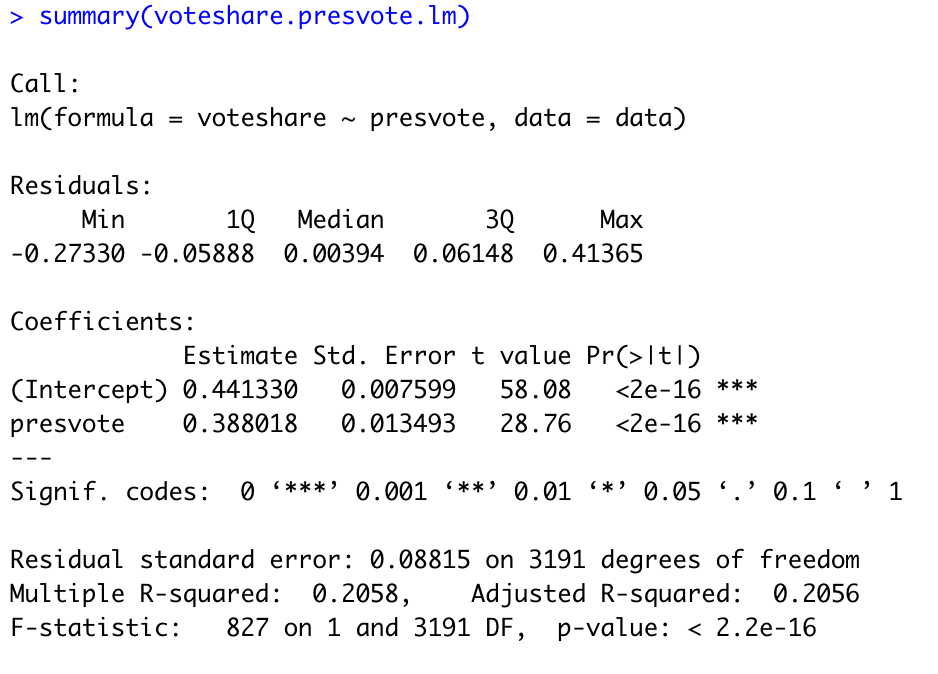
\includegraphics{PS3 Q3 Regression.png}

\newpage
		\item Make a scatterplot of the two variables and add the regression line. 
\noindent We use the \texttt{ggplot()} function to create a scatterplot where \texttt{voteshare} is on the y axis and \texttt{presvote} is on the x axis.
\begin{lstlisting}
ggplot(data, aes(x=presvote, y=voteshare))+
geom_point()+
geom_smooth(method=lm)
\end{lstlisting}
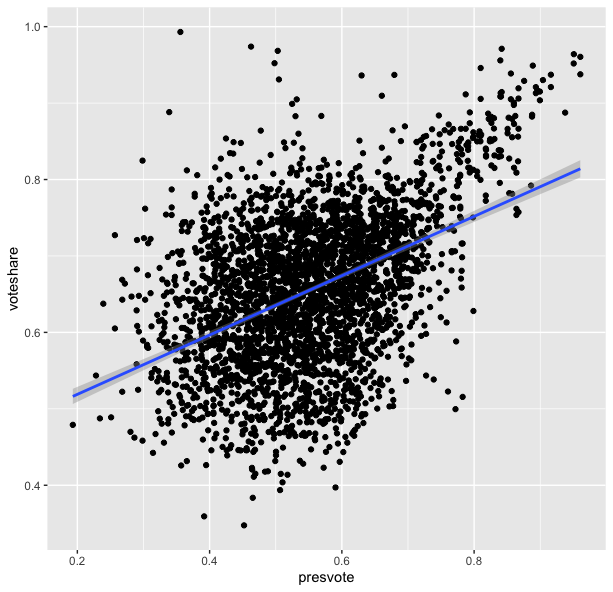
\includegraphics[width=\textwidth]{Scatterplot XPresvote YVoteshare.png}
\newpage

		\item Write the prediction equation.
\\\\
\noindent As in Questions 1 and 2, the prediction equation is given by \texttt{y = b0 + b1x}, where b0 is the intercept of the regression and b1, the coefficient of x, is the \texttt{difflog} value in the regression.
\\\\
\noindent As we can see in Table 3, the value for \texttt{presvote} (b1) is 0.388 and the value of the intercept (b0) is 0.441.
\\\\
\noindent Therefore, the prediction equation is:
\\\\
\noindent \texttt{y = 0.388x + 0.441}.
		
	\end{enumerate}
	

\newpage	
\section*{Question 4}
\noindent The residuals from part (a) tell us how much of the variation in \texttt{voteshare} is $not$ explained by the difference in spending between incumbent and challenger. The residuals in part (b) tell us how much of the variation in \texttt{presvote} is $not$ explained by the difference in spending between incumbent and challenger in the district.
	\begin{enumerate}
		\item Run a regression where the outcome variable is the residuals from Question 1 and the explanatory variable is the residuals from Question 2.	
\\\\
\noindent We run a regression where the outcome variable (y) is the residuals from Question 1 (\texttt{residualsVoteshareDifflog}) and the explanatory variable (x) is the residuals from Question 2 (\texttt{residualsPresvoteDifflog}). 
\\We save it in a variable called \texttt{rVoteshareDifflog.rPresvoteDifflog.lm}. Finally, we use the stargazer function to generate the following Latex output.

\begin{lstlisting}
rVoteshareDifflog.rPresvoteDifflog.lm <- lm(residualsVoteshareDifflog ~ residualsPresvoteDifflog, data = data)
summary(rVoteshareDifflog.rPresvoteDifflog.lm)
stargazer(rVoteshareDifflog.rPresvoteDifflog.lm, type='latex', summary= FALSE)
\end{lstlisting}
\begin{table}[!htbp] \centering 
  \caption{} 
  \label{} 
\begin{tabular}{@{\extracolsep{5pt}}lc} 
\\[-1.8ex]\hline 
\hline \\[-1.8ex] 
 & \multicolumn{1}{c}{\textit{Dependent variable:}} \\ 
\cline{2-2} 
\\[-1.8ex] & residualsVoteshareDifflog \\ 
\hline \\[-1.8ex] 
 residualsPresvoteDifflog & 0.257$^{***}$ \\ 
  & (0.012) \\ 
  & \\ 
 Constant & $-$0.000 \\ 
  & (0.001) \\ 
  & \\ 
\hline \\[-1.8ex] 
Observations & 3,193 \\ 
R$^{2}$ & 0.130 \\ 
Adjusted R$^{2}$ & 0.130 \\ 
Residual Std. Error & 0.073 (df = 3191) \\ 
F Statistic & 476.975$^{***}$ (df = 1; 3191) \\ 
\hline 
\hline \\[-1.8ex] 
\textit{Note:}  & \multicolumn{1}{r}{$^{*}$p$<$0.1; $^{**}$p$<$0.05; $^{***}$p$<$0.01} \\ 
\end{tabular} 
\end{table}
\newpage
\noindent Below is a screenshot of the output from the console in R Studio of the regression model.
\\\\
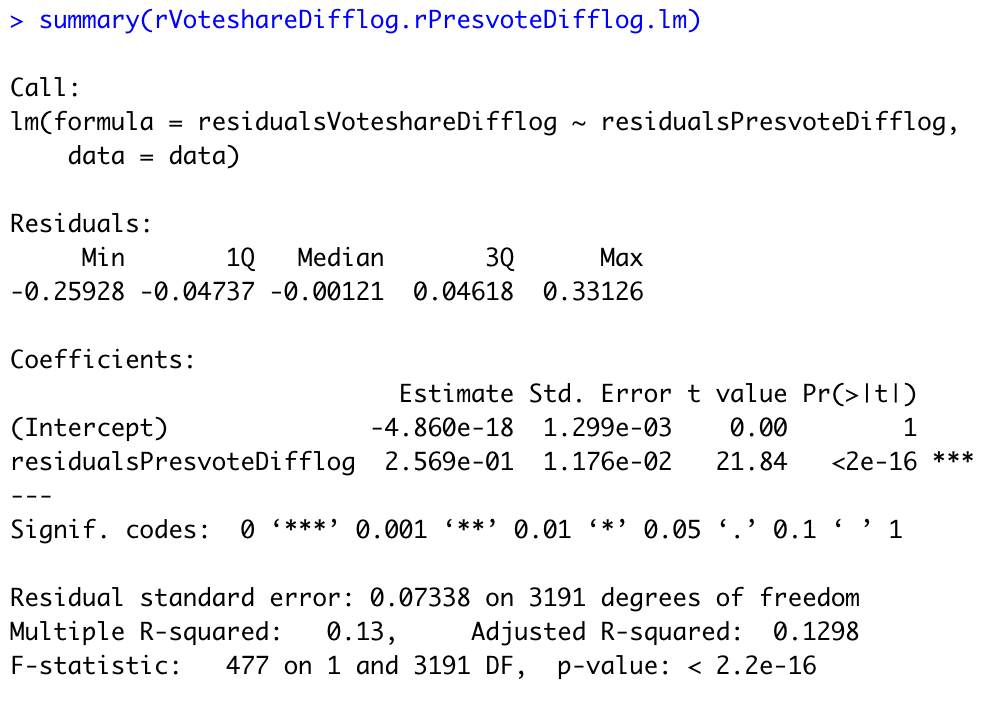
\includegraphics{PS3 Q4 Regression.png}
\\\\
\noindent The residuals of the regression are the difference between the observed and predicted values of the regression. We can see a min residual value of -0.25928, and a max residual value of 0.33126. The median residual value is -0.00121, which is quite near 0.
\\\\
\noindent The p-value for the intercept at 1 is extremely high. This suggests that it is very unlikely to be signficant to say the intercept value is 0. 
\\\\
\noindent The Multiple R squared value is 0.13, which suggests that around 13 percent of the variance of \texttt{ResidualsVoteshareDifflog} is explained by \texttt{ResidualsPresvoteDifflog}.

\newpage
		\item Make a scatterplot of the two residuals and add the regression line.
\\\\		
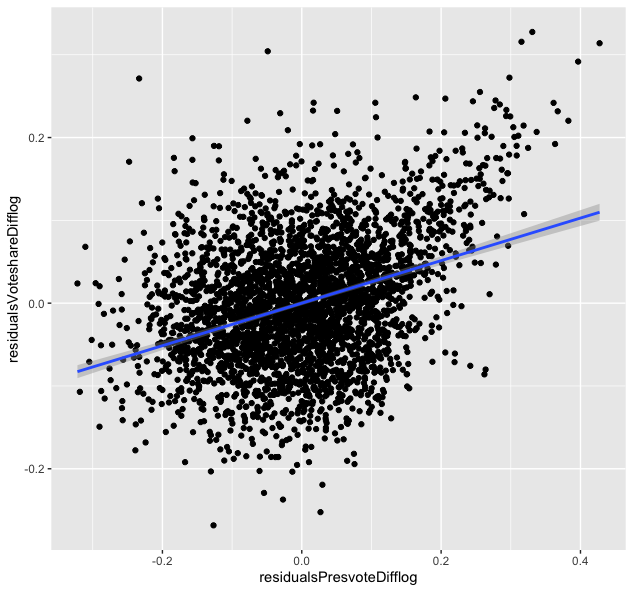
\includegraphics[width=\textwidth]{Scatterplot XResidualsPresvoteDifflog YResidualsVoteshareDifflog.png}
\newpage		
		\item Write the prediction equation.
\\\\
\noindent As in the previous questions, the prediction equation is given by \texttt{y = b0 + b1x}, where b0 is the intercept of the regression and b1, the coefficient of x, is the \texttt{residualsVoteshareDifflog} value in the regression.
\\\\
\noindent As we can see in Table 4, the value for \texttt{residualsPresvoteDifflog} (b1) is 0.257 and the value of the intercept (b0) is -0.000, or 0.
\\\\
\noindent Therefore, the prediction equation is:
\\\\
\noindent \texttt{y = 0.257x - 0.000}
\\\\
\noindent Or, more simply:
\\\\
\noindent \texttt{y = 0.257x}
	\end{enumerate}
	
	\newpage	

\section*{Question 5}
\noindent What if the incumbent's vote share is affected by both the president's popularity and the difference in spending between incumbent and challenger? 
	\begin{enumerate}
		\item Run a regression where the outcome variable is the incumbent's \texttt{voteshare} and the explanatory variables are \texttt{difflog} and \texttt{presvote}.	
\\\\
\noindent We run a regression where the outcome variable (y) is the incumbent's \texttt{voteshare} and the explantory variables (x) are \texttt{difflog} and \texttt{presvote}. We save it a variable called \texttt{voteshare.difflog.presvote.lm}. Finally, we use the \texttt{stargazer} function to yield Latex output as follows:
\begin{lstlisting}
voteshare.difflog.presvote.lm <- lm(voteshare ~ difflog + presvote, data = data)
summary(voteshare.difflog.presvote.lm)
stargazer(voteshare.difflog.presvote.lm, type='latex', summary= FALSE)
\end{lstlisting}

\begin{table}[!htbp] \centering 
  \caption{} 
  \label{} 
\begin{tabular}{@{\extracolsep{5pt}}lc} 
\\[-1.8ex]\hline 
\hline \\[-1.8ex] 
 & \multicolumn{1}{c}{\textit{Dependent variable:}} \\ 
\cline{2-2} 
\\[-1.8ex] & voteshare \\ 
\hline \\[-1.8ex] 
 difflog & 0.036$^{***}$ \\ 
  & (0.001) \\ 
  & \\ 
 presvote & 0.257$^{***}$ \\ 
  & (0.012) \\ 
  & \\ 
 Constant & 0.449$^{***}$ \\ 
  & (0.006) \\ 
  & \\ 
\hline \\[-1.8ex] 
Observations & 3,193 \\ 
R$^{2}$ & 0.450 \\ 
Adjusted R$^{2}$ & 0.449 \\ 
Residual Std. Error & 0.073 (df = 3190) \\ 
F Statistic & 1,302.947$^{***}$ (df = 2; 3190) \\ 
\hline 
\hline \\[-1.8ex] 
\textit{Note:}  & \multicolumn{1}{r}{$^{*}$p$<$0.1; $^{**}$p$<$0.05; $^{***}$p$<$0.01} \\ 
\end{tabular} 
\end{table} 		
\newpage
\noindent Attached is a screenshot of the output from the R studio console which summarises the regression model.
\\\\
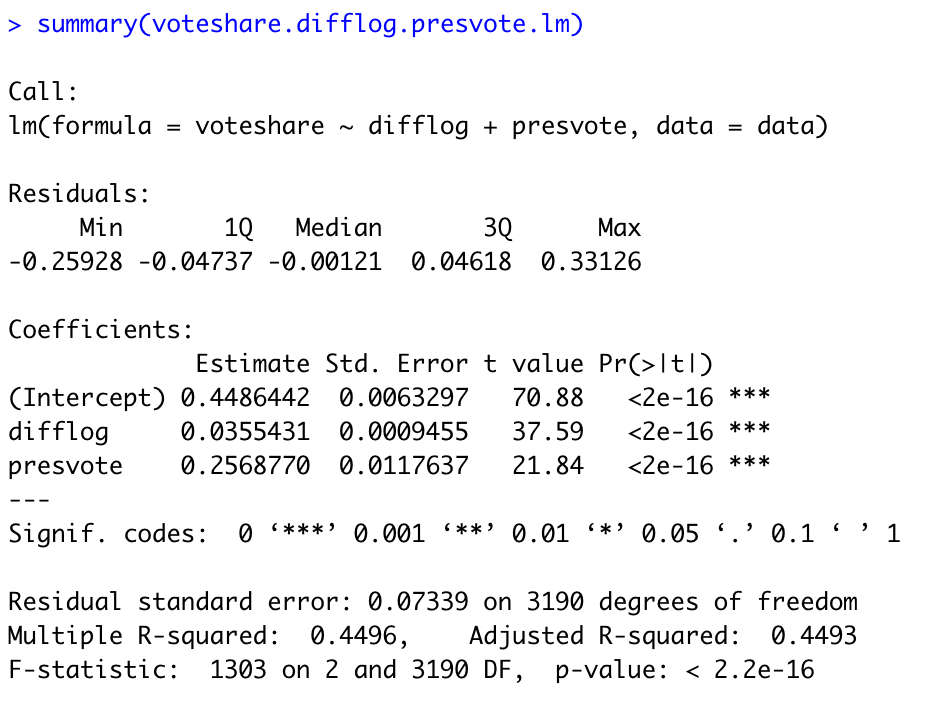
\includegraphics{PS3 Q5 Regression.png}
\newpage
		\item Write the prediction equation.
\\\\
\noindent Since we have two explanatory variables, \texttt{difflog} and \texttt{presvote}, we are running a multiple linear regression as opposed to a simple linear regression in the previous 4 questions. As such, we use a different prediction equation to account for the extra explanatory variable.
\\\\
\noindent We use the following equation:
\\\\
\noindent \texttt{y = b0 + b1x1 + b2x2}
\\\\
\noindent Where y is the outcome variable \texttt{voteshare}, b0 is the intercept of model or the constant, b1 is the coefficient of the first explanatory variable \texttt{difflog}, x1 is the value of the first explanatory variable \texttt{difflog}, b2 is the coefficient of the second explantory variable \texttt{presvote} and x2 is the value of the second explantory variable \texttt{presvote}.
\\\\
\noindent In our regression model, as seen from Table 5, the coefficient of \texttt{difflog} is 0.036, the coefficient of \texttt{presvote} is 0.257 and the constant/intercept is 0.449.
\\\\
\noindent  Therefore, our prediction equation for this model is:
\\\\
\noindent \texttt{y = (0.036)x1 + (0.257)x2 + 0.449}
\\\\
\noindent Or:
\\\\
\noindent \texttt{voteshare = (0.036)difflog + (0.257)presvote + 0.449}

\vspace{1cm}
\newpage
		\item What is it in this output that is identical to the output in Question 4? Why do you think this is the case?
\\\\

\noindent We can see that the coefficient estimate, standard error, t-value and p-value of the \texttt{presvote} variable in Question 5 are identical to the coefficient estimate, standard error, t-value and p-value of the Question 4 regression of residuals of \texttt{presvote} and the residuals of \texttt{difflog}.
\\\\
\noindent The regression in Question 4 plots the residuals of \texttt{Voteshare} against \texttt{Difflog} against the residuals of \texttt{Presvote} against \texttt{Difflog}. This regression plots the unexplained variation in \texttt{voteshare.difflog.lm} against the unexplained variation in \texttt{presvote.difflog.lm} to see if there is a relationship between the two unexplained variations. The plot in Question 4 measures the amount of variation \texttt{voteshare} that is explained by presvote without any influence from the \texttt{difflog} variable. It shows, essentially, how much voteshare is influence by \texttt{presvote} on it's own, without \texttt{difflog}.
\\\\
\noindent This is the same thing that the regression in Question 5 shows. The regression separates the two variables and shows how much variance in \texttt{voteshare} is explained by \texttt{difflog} on it's own, namely a 0.036 increase in \texttt{voteshare} for a one unit increase in \texttt{difflog}. 
\\\\
\noindent As \texttt{difflog} and \texttt{presvote} are separated in the multiple linear regression of Question 5, the coefficient of \texttt{presvote} in Question 5 therefore shows how much variation is explained by \texttt{presvote} without any influence from \texttt{difflog}. This means that a 1 unit increase in \texttt{presvote} on its own will result in a 0.257 increase in \texttt{voteshare}.
\\\\
\noindent The min, Q1, median, Q3 and max values of the residuals of Question 4 are also identical to the min, Q1, median, Q3 and max values of the residuals of Question 5, for the same reasons.  	

	\end{enumerate}




\end{document}